\documentclass[fleqn]{article}
\oddsidemargin 0.0in
\textwidth 6.0in
\thispagestyle{empty}
\usepackage{import}
\usepackage{amsmath}
\usepackage{graphicx}
\usepackage{flexisym}
\usepackage{calligra}
\usepackage{amssymb}
\usepackage{bigints} 
\usepackage[english]{babel}
\usepackage[utf8x]{inputenc}
\usepackage{float}
\usepackage[colorinlistoftodos]{todonotes}


\DeclareMathAlphabet{\mathcalligra}{T1}{calligra}{m}{n}
\DeclareFontShape{T1}{calligra}{m}{n}{<->s*[2.2]callig15}{}
\newcommand{\scriptr}{\mathcalligra{r}\,}
\newcommand{\boldscriptr}{\pmb{\mathcalligra{r}}\,}

\definecolor{hwColor}{HTML}{442020}

\begin{document}

  \begin{titlepage}

    \newcommand{\HRule}{\rule{\linewidth}{0.5mm}}

    \center

    \begin{center}
      
\includegraphics[height=11cm, width=11cm]{asu.png}
    \end{center}

    \vline

    \textsc{\LARGE Classical Parts/Field/Matter III}\\[1.5cm]

    \HRule \\[0.5cm]
    { \huge \bfseries Midterm Exam 1}\\[0.4cm] 
    \HRule \\[1.0cm]

    \textbf{Behnam Amiri}

    \bigbreak

    \textbf{Prof: Samuel Teitelbaum}

    \bigbreak

    \textbf{{\large \today}\\[2cm]}

    \vfill

  \end{titlepage}


  \begin{itemize}
    \item This exam is available all weekend, but should take you 4-6 hours to complete.
    \item Your solutions must be uploaded to Canvas just as you do with homework.
    \item The exam should be taken without the use of internet (aside from Canvas materials, and email
    in the event that you have questions during the exam).
    \item The only allowed materials are: Griffiths textbook, your math methods textbook, any materials
    on Canvas, and your own hand-written or hand-typed notes.
    \item Do not discuss the midterm problems with anyone until after Febuary $23, ~ 2022$.
    \item If you get stuck on math, explain the physics as well as you can.
  \end{itemize}

  \pagebreak

  \begin{enumerate}
    \item \textbf{Problem 1 [20 points]}
    \begin{enumerate}
      \item Derive the charge continuity equation directly from Maxwell’s equations (7.40).

        % \textcolor{hwColor}{
        %   \\
        % }
      
      \item Suppose there is a charge current density $\mathcal{J}=Cx ~ \hat{x}$ within some region of space. Find the
      charge density $\rho(r, t)$ at the origin $r=0$ at some later time $t$, assuming that $\rho(0, 0)=0$.

        % \textcolor{hwColor}{
        %   \\
        % }
      
    \end{enumerate}


    \item \textbf{Problem 2 [20 points]} A toroid with a current $I$ and a total of n windings is placed in an uniform
    electric field $\mathcal{E}=E ~ \hat{z}$, which points along the axis of symmetry of the toroid. The toroid has a radius
    and rectangular cross section of dimensions shown in the figure.

      \begin{figure}[h!]
        \centering
        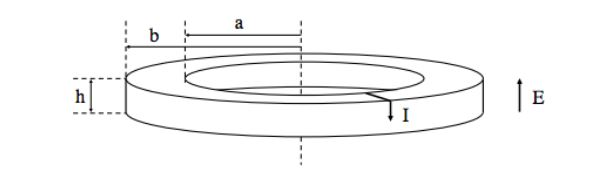
\includegraphics[height=4cm, width=8cm]{One.JPG}
      \end{figure}

      \begin{enumerate}
        \item Determine the Poynting vector everywhere in space. Use the standard cylindrical coordinates
        with axes $\hat{s}$, $\hat{\phi}$, $\hat{z}$.

          % \textcolor{hwColor}{
          %   \\
          % }

        \item Determine the total flux of field energy into the toroid by integrating the Poynting vector.

          % \textcolor{hwColor}{
          %   \\
          % }

        \item Determine the total linear momentum stored in the fields.

          % \textcolor{hwColor}{
          %   \\
          % }

        \item Determine the total angular momentum stored in the fields.

          % \textcolor{hwColor}{
          %   \\
          % }

        \item Qualitatively, what happens to the toroid when the E field is reduced to zero?

          % \textcolor{hwColor}{
          %   \\
          % }

      \end{enumerate}

    \item \textbf{Problem 3 [20 points]} 
    Two infinite, electrically neutral wires are parallel to each other and each carries a current $I$ flowing
    in the $\hat{z}$ direction. The axes of the wires pass through the points $\pm d\hat{x}$ (hence they are separated by
    a distance $2d$).
    \begin{enumerate}
      \item Determine the force per unit length acting on the wire passing through $+d\hat{x}$ by making use of
      the Maxwell stress tensor. Make sure that you get the correct direction of the force.

        % \textcolor{hwColor}{
        %   \\
        % }


      \item Confirm the result in part (a) by doing the easier calculation (i.e. use the Lorentz force law).
      The following integral might be helpful for part (a):
      $$
        \int\limits_{-\infty}^{+\infty} ~ \dfrac{y^2}{\left(y^2+d^2\right)^2} ~ dy=\dfrac{\pi}{2d} 
      $$

        % \textcolor{hwColor}{
        %   \\
        % }

    \end{enumerate}

    \item \textbf{Problem 4 [20 points]} The electric field of an elliptically polarized EM wave in vacuum is formed by the superposition
      $$
        E(r,t)=E_y ~ sin(ax-wt) ~ \hat{y}+E_z ~ cos(ax-wt) ~ \hat{z}
      $$
      where $a$ is a positive constant.
      \begin{enumerate}
        \item What is the direction that the wave travels, and what is its wavelength?

          % \textcolor{hwColor}{
          %   \\
          % }

        \item Determine the radiation pressure carried by the field by deriving the Maxwell stress tensor for
        the field.

          % \textcolor{hwColor}{
          %   \\
          % }
        
      \end{enumerate}

    \item \textbf{Problem 4 [20 points]}
    \begin{enumerate}
      \item State the three laws of geometrical optics that were derived in Griffiths. \emph{Hint: recall that they
      concern relationships between angles of incidence, reflection, and transmission.}

        % \textcolor{hwColor}{
        %   \\
        % }


      \item State three important assumptions about the materials that were used in deriving the above laws.

        % \textcolor{hwColor}{
        %   \\
        % }


      \item Explain what the “Brewster angle” is in one sentence.

        % \textcolor{hwColor}{
        %   \\
        % }
      
    \end{enumerate}

  \end{enumerate}

\end{document}
